\section{Markov Chains}
\begin{framed}
    A \textbf{Markov Chain} over $\sS \defeq \{0, \dots, n-1\}$, is a sequence $(X_t)_{t \in \Nat_0} \in \sS$, such that the \textbf{Markov property}: $X_{t+1} \perp X_{0:t-1} \mid X_t$ is satisfied. 
\end{framed}
It is \textbf{time-homogeneous} if there is a \textbf{transition function}: $p(x' \mid x) \defeq \Pr{X_{t+1} = x' \mid X_t = x}$, with \textbf{transition matrix} as $\left(x_j \mid x_i \right)_{i, j = 1}^n$. Each row sums up to 1. \\
The state of a MC at $t$ is a probability distribution $\vq_t \in \in \R^{1 \times \card{\sS}}$. We can write: $\vq_{t+k} = \vq_t \mP^k$.
\begin{framed}
    A distribution $\pi$ is \textbf{stationary} iff\\ $\pi(x) = \sum_{x' \in S} p(x \mid x') \pi(x')$ equivalently $\vpi = \vpi \mP$.
\end{framed}
A MC is \textbf{irreducible} if every state is reachable from any state with positive probability.
\begin{framed}
    A MC is \textbf{ergodic} iff there exists a $t \in \Nat_0$ such that for any $x, x' \in S$ we have: $p^{(t)}(x' \mid x) > 0$. Equivalently:
    for some $t \in \Nat_0$ all entries of $\mP^t$ are strictly positive \\
    or that the MC is irreducible and aperiodic.
\end{framed}
Irreducible MC $\rightarrow$ ergodic MC use: $\mP' = \frac{1}{2}\mP + \frac{1}{2}\mI$
\begin{framed}
    An ergodic MC has a unique stat. dist. $\pi$ (with full support) and $\lim_{t\to\infty} q_t = \pi$, independently of $q_0$.
\end{framed}
\begin{framed}
    A MC satisfies the \textbf{detailed balance equation} w.r.t. $\pi$ iff $\pi(x) p(x' \mid x) = \pi(x') p(x \mid x')$, for any $x, x' \in S$. We call such a MC \textbf{reversible} w.r.t. $\pi$.
\end{framed}
If MC is reversible w.r.t. $\pi$, then $\pi$ is a stat. dist.
\begin{framed}
    \textbf{Ergodic theorem} For an ergodic MC and a stat. dist. $\pi$ as well as $f : \sS \to \R$:
    $\frac{1}{n} \sum_{i=1}^n f(x_i) \almostsurely \sum_{x \in S} \pi(x) f(x) = \E[x \sim \pi]{f(x)}$, for $n\to\infty$ where $x_i \sim X_i \mid x_{i-1}$.
\end{framed}
\textbf{Acceptance distribution (Metropolis-Hastings)}: $\Bern{\alpha(\vxp \mid \vx)}$ where $\alpha(\vxp \mid \vx) \defeq \min \braces*{1, \frac{q(\vxp) r(\vx \mid \vxp)}{q(\vx) r(\vxp \mid \vx)}}$ to decide whether to follow the proposal yields a Markov chain with stationary distribution $p(\vx) = \frac{1}{Z} q(\vx)$.
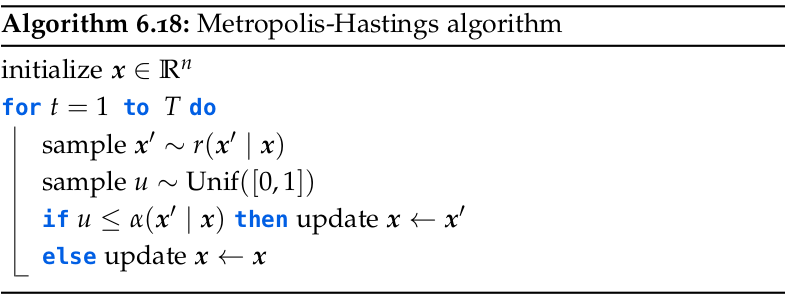
\includegraphics[width=0.98\linewidth, trim={0 0 5cm 0}]{images/Metropiolis_Hasting.png}
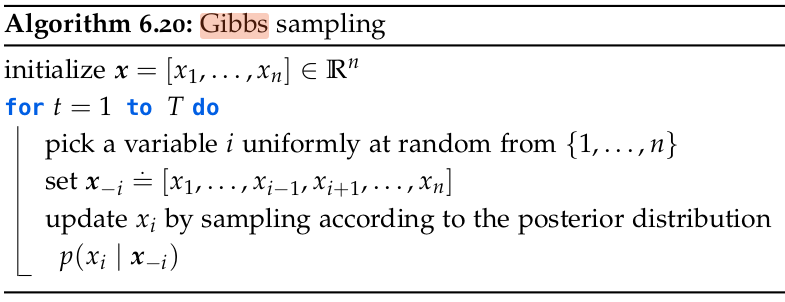
\includegraphics[width=0.98\linewidth]{images/Gibbs_Sampling.png} 
The stationary distribution of the simulated Markov chain is $p(\vx)$.
A \textbf{Gibbs distribution} is a continuous distribution $p$ whose PDF is of the form $p(\vx) = \frac{1}{Z} \exp(- f(\vx))$. $f$ is also called an \textbf{energy function}.
When the energy function $f$ is convex, its Gibbs distribution is called \textbf{log-concave distribution}. Can write: $\alpha(\vxp \mid \vx) = \min \braces*{1, \frac{r(\vx \mid \vxp)}{r(\vxp \mid \vx)} \exp(f(\vx) - f(\vxp))}$. \\
For $p(\vx) \propto \exp(-f(\vx))$: $\S{p(\vx)} = f(\vx) + \log Z$
\begin{framed}
    \textbf{Langevin Dynamics}: Shift the proposal distribution perpendicularly to the gradient of the energy function: $r(\vxp \mid \vx) = \N[\vxp]{\vx - \eta_t \grad f(\vx)}{2 \eta_t \mI}$.
\end{framed}
